\begin{figure}[H]
\centering
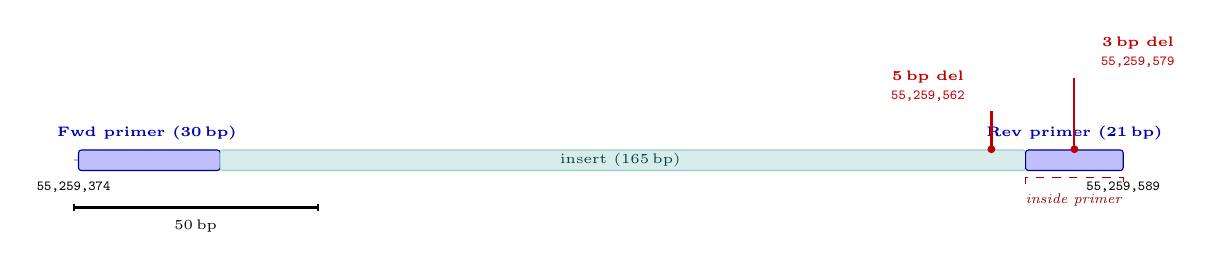
\begin{tikzpicture}[x=0.062cm, y=1cm, font=\footnotesize]

  % -------------------------------------------------------
  % Coordinates (bp offset from amplicon start 55,259,374)
  % Fwd primer : 1  -- 30   (55,259,375--55,259,404)
  % Insert     : 30 -- 195
  % Rev primer : 195 -- 215 (55,259,569--55,259,589)
  % 5 bp del   : 188        (55,259,562)  -- 7 bp before rev primer
  % 3 bp del   : 205        (55,259,579)  -- inside rev primer
  % -------------------------------------------------------

  % Backbone
  \draw[gray!50, thick] (0, 0) -- (215, 0);

  % Forward primer
  \filldraw[fill=blue!25, draw=blue!55!black, rounded corners=1pt]
    (1, -0.13) rectangle (30, 0.13);
  \node[above, font=\tiny\bfseries, blue!70!black] at (15, 0.13)
    {Fwd primer (30\,bp)};

  % Insert
  \filldraw[fill=teal!15, draw=teal!40, rounded corners=1pt]
    (30, -0.13) rectangle (195, 0.13);
  \node[font=\tiny, teal!50!black] at (112, 0) {insert (165\,bp)};

  % Reverse primer
  \filldraw[fill=blue!25, draw=blue!55!black, rounded corners=1pt]
    (195, -0.13) rectangle (215, 0.13);
  \node[above, font=\tiny\bfseries, blue!70!black] at (205, 0.13)
    {Rev primer (21\,bp)};

  % Amplicon boundary labels
  \node[below, font=\tiny] at (0,   -0.15) {\texttt{55,259,374}};
  \node[below, font=\tiny] at (215, -0.15) {\texttt{55,259,589}};

  % ---- 5 bp deletion (pos 188, just outside rev primer) ----
  \draw[red!75!black, thick] (188, 0.14) -- (188, 0.62);
  \filldraw[red!75!black] (188, 0.14) circle (1.2pt);
  \node[above, font=\tiny\bfseries, red!75!black, align=center] at (175, 0.62)
    {5\,bp del\\[1pt]\texttt{55,259,562}};

  % ---- 3 bp deletion (pos 205, inside rev primer) ----
  \draw[red!75!black, thick] (205, 0.14) -- (205, 1.05);
  \filldraw[red!75!black] (205, 0.14) circle (1.2pt);
  \node[above, font=\tiny\bfseries, red!75!black, align=center] at (218, 1.05)
    {3\,bp del\\[1pt]\texttt{55,259,579}};

  % Annotation: "inside primer" brace for 3 bp del
  \draw[red!60!black, dashed, thin]
    (195, -0.30) -- (195, -0.22) -- (215, -0.22) -- (215, -0.30);
  \node[below, font=\tiny, red!60!black] at (205, -0.30)
    {\textit{inside primer}};

  % Scale bar
  \draw[thick] (0, -0.60) -- (50, -0.60);
  \draw[thick] (0, -0.55) -- (0,  -0.65);
  \draw[thick] (50,-0.55) -- (50, -0.65);
  \node[below, font=\tiny] at (25, -0.63) {50\,bp};

\end{tikzpicture}
\caption{Amplicon~3 (exon~21) primer layout and positions of the two Mutect2
  PASS deletion calls. The forward primer (blue, left) and reverse primer (blue,
  right) were localised by BLAST. The 3\,bp deletion at chr7:55{,}259{,}579
  falls \emph{inside} the reverse primer binding region, confirming it as a
  primer-end artefact. The 5\,bp deletion at chr7:55{,}259{,}562 lies 7\,bp
  upstream of the reverse primer and is at the primer--insert junction, where
  polymerase slippage is a known source of apparent boundary deletions. Neither
  call represents a true somatic variant; both would be eliminated by running
  \texttt{ivar trim} before variant calling.}
\label{fig:exon21-primer-artefact}
\end{figure}
